\documentclass{beamer}

\mode<presentation>
{
	\usetheme{Warsaw}
	\setbeamercovered{transparent}
}

\usepackage[utf8]{inputenc}
\usepackage[czech]{babel}
\usepackage{palatino}
\usepackage{graphicx}


%%%%%%%%%%%%%%%%%%%%%%%%%%%%%%%%%%%%%%%%%%%%%%%%%%%%%%%%%%%%%%%%%%%%%%%%%%%%%%
%%%%

\newcommand{\frameWithTitleImage}[2]
{
	\begin{frame}
		\frametitle{#1}
		\begin{center}
		\includegraphics[width=\textwidth,height=0.8\textheight,keepaspectratio]{#2}
		\end{center}
	\end{frame}
}

\newcommand{\frameWithImage}[1]
{
	\begin{frame}
		\begin{center}
		\includegraphics[width=\textwidth,height=0.8\textheight,keepaspectratio]{#1}
		\end{center}
	\end{frame}
}

\newcommand{\frameWithTitle}[1]
{
	\begin{frame}
		\begin{center}
		\textbf{\Large{#1}}
		\end{center}
	\end{frame}
}


%%%%%%%%%%%%%%%%%%%%%%%%%%%%%%%%%%%%%%%%%%%%%%%%%%%%%%%%%%%%%%%%%%%%%%%%%%%%%%
%%%%

\title[Interpret grafových algoritmů]{\normalsize{Diplomová práce\\Interpret grafových algoritmů}}
\author{Bc. Michal Turek}
\institute{FEL ČVUT v Praze}
\date{\small{leden 2010}}

\begin{document}

\begin{frame}
	\titlepage
	\begin{center}
	\small{Vedoucí práce: RNDr. Marko Genyk-Berezovskyj}
	\end{center}
\end{frame}


\begin{frame}
	\frametitle{Cíl práce}
	\begin{itemize}
	\item Vytvoření prostředí pro výzkum algoritmů \textit{difúze} (rozpoznávání obrazů)
	\item Přeneseně: Vývojové prostředí pro ladění a vizualizace grafových algoritmů
	\end{itemize}

	\begin{center}
	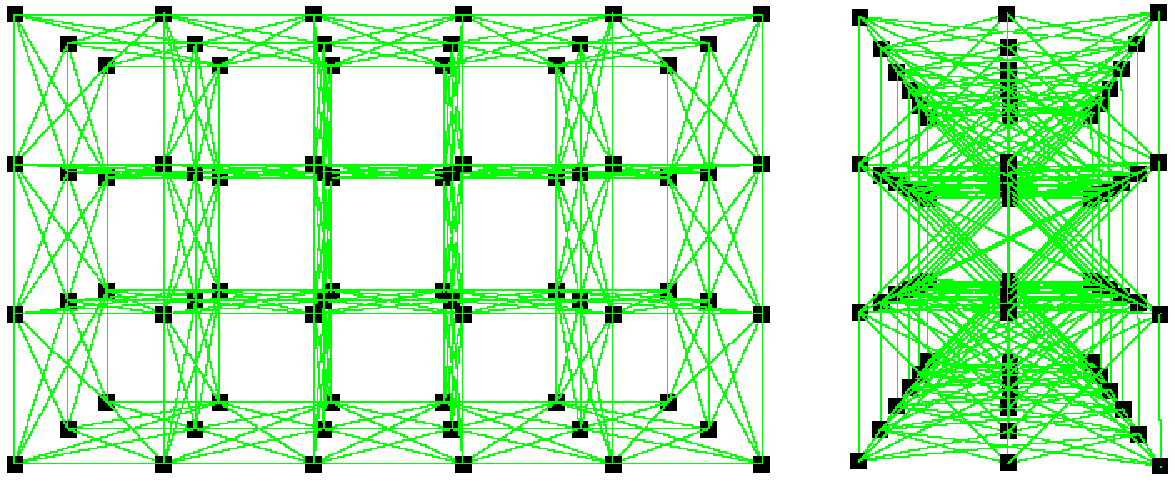
\includegraphics[width=7cm]{../text/img/graf_difuze.pdf}
	\end{center}
\end{frame}


\begin{frame}
	\frametitle{Zadání práce}
	\begin{itemize}
	\item Návrh nového programovacího jazyka
		\begin{itemize}
		\item Snadný zápis grafových algoritmů
		\item Syntaxe jazyka C
		\end{itemize}
	\item Vytvoření interpretu pro příkazovou řádku
	\item Vytvoření grafického uživatelského rozhraní
		\begin{itemize}
		\item Programátorsky zaměřený textový editor
		\item Spuštění a krokování algoritmu
		\item Vizualizace grafu ve 3D
		\end{itemize}
	\end{itemize}
\end{frame}


\begin{frame}
	\frametitle{Implementační prostředí}
	\begin{itemize}
	\item Jazyk C++, STL, GNU Bison, perlovské skripty
	\item Qt, OpenGL
	\item Code::Blocks, Qt Creator, Makefile
	\end{itemize}
\end{frame}


\begin{frame}
	\frametitle{Interpret}
	\begin{itemize}
	\item Datové typy a operace
		\begin{itemize}
		\item Double dispatching pattern
		\end{itemize}
	\item Vykonávání skriptu
		\begin{itemize}
		\item Rekurzivní procházení AST
		\end{itemize}
	\item Reprezentace grafů
		\begin{itemize}
		\item Hrana ukládá ukazatele na počáteční a koncový vrchol
		\item Vrchol ukládá ukazatele na incidující hrany
		\end{itemize}
	\item Paměťový management
		\begin{itemize}
		\item Chytré ukazatele na bázi čítání referencí
		\end{itemize}
	\end{itemize}
\end{frame}


\frameWithTitleImage{Okno grafické aplikace}{../text/img/screenshot.png}


\begin{frame}
	\frametitle{Grafická aplikace}
	\begin{itemize}
	\item Oddělení CLI a GUI
		\begin{itemize}
		\item Dva nezávislé programy
		\item Návrhový vzor továrna
		\end{itemize}
	\item Krokování a debugging
		\begin{itemize}
		\item Synchronizační prostředky vláken
		\end{itemize}
	\item Propojení skriptu a vizualizací
		\begin{itemize}
		\item Zabudované funkce
		\item Jednotné rozhraní pro komunikaci
		\item Qt signály a sloty
		\end{itemize}
	\end{itemize}
\end{frame}


\frameWithTitleImage{Rychlost vykonávání ve srovnání s jazykem Perl}{../text/img/benchmark.pdf}


\begin{frame}
	\frametitle{Shrnutí}
	\begin{itemize}
	\item Všechny požadavky ze zadání splněny
	\item Věci navíc
		\begin{itemize}
		\item Podporován libovolný typ grafů
		\item Výkonný debugger
		\item Netriviální editor
		\item Aplikace je přenositelná mezi operačními systémy
		\end{itemize}
	\item Budoucnost
		\begin{itemize}
		\item Zvýšení rychlosti interpretace
		\item Nové zabudované funkce
		\end{itemize}
	\end{itemize}
\end{frame}


\frameWithTitle{Otázky?}
\frameWithTitle{Děkuji za pozornost!}

\end{document}
